% 量子力学

这里讨论的是非相对论量子力学,只适用于低速微观粒子.

\subsection{波函数}

\begin{figure}[ht]
\centering
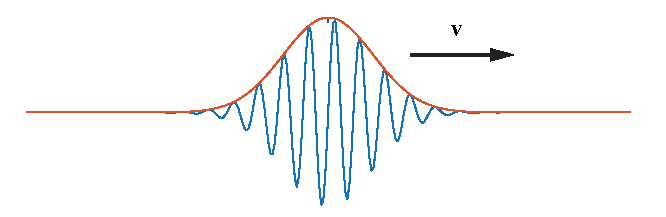
\includegraphics[width=12cm]{./figures/QM01.pdf}
\caption{蓝线是一维波函数/绳子的形状,橙线是振幅.某个位置的振幅越大,粒子就越有可能出现在该位置.图中的形状叫做波包,一般来说波函数可以是几乎任何形状.} \label{QM0_fig1}
\end{figure}

这里只讨论一维的情况,即粒子沿直线运动.经典力学中用位置关于时间的函数描述一个粒子的运动,而量子力学中用波函数描述.波函数是一个关于位置和时间的函数,例如一条紧绷的绳子(或弦)上的波动,绳子的高度 y 是关于位置 x 和时间 t 的函数.某个位置震动的幅度的平方就是粒子在这个位置出现的概率.经典力学中,给出粒子初始的位置和速度和势能,它将按照牛顿第二定律运动.量子力学中,给出粒子的初始波函数,波函数将按照含时薛定谔方程变化,把势能和某个时刻的波函数代入薛定谔方程,就可以解出任意时刻的波函数(这类方程并不是数的方程,而是函数的方程,所以解出的是函数,而不是数).薛定谔方程是量子力学的公设之一,就像牛顿三定律是牛顿力学的公设.量子力学中,粒子都用波表示,是因为许多实验发现微观粒子(如电子,质子,中子)具有一些波的性质,这就是著名的波粒二象性.
(注释1:波函数和绳子的运动方式相似但不完全相同.注释2:波函数的值是复数,粒子出现在某点的概率是复数模长的平方.这里为了简单暂时使用实数,可以看做是复数的实部.)

\subsection{波包}
即使粒子的位置一般不能精确确定,我们往往也能确定其大致范围(例如实验物理学家往往知道某粒子在实验室而不在月球),所以波函数往往只有在一定范围内不为零(我们只能在一定空间范围内测到检测到粒子).将振幅关于位置的函数画出来,其形状往往像一个包(越靠近中间,检测到粒子的概率越大),我们称为波包.

\subsection{自由粒子}

\begin{figure}[ht]
\centering
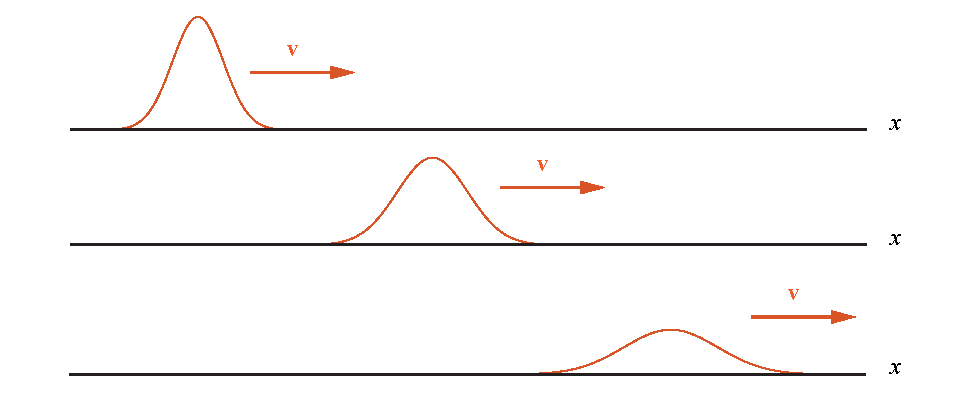
\includegraphics[width=14cm]{./figures/QM02.pdf}
\caption{对应自由粒子的波包.注意图中波包仅画出了振幅,没画出上一张图中的具体的波动形状.} \label{QM0_fig2}
\end{figure}

先看不受力的粒子(叫自由粒子),在经典力学中,粒子不受力时静止或者做匀速运动.量子力学中,若粒子不受力(势能处处为常数)且初始时波函数为波包且具有初速度,波包中心就会匀速运动,但同时波包会扩散(越变越宽,越变越矮).想象一根紧绷的绳子的一端突然迅速上下抖了几下又停下来,那么将产生一个波包将从绳的一段传到另一端(不同的是绳子上的波包形状不会变化).如果波包开始是静止,那么波包只会在原地扩散.

当我们回到宏观中,把波包近似成质点,那波包的中心就是质点的位置,中心速度就是质点的速度.(小时物理百科的 logo 就是自由高斯波包!)

\subsection{无限深势阱}
经典力学中,若质点在两面墙之间不停反弹,与墙不断发生完全弹性碰撞(碰撞后速度大小不变).如果用势能描述,就是墙之间的势能为零(或常数),墙和墙外的势能为无限大.这种势能叫做无限深势阱.量子力学中,波包在无限深势阱中同样一边来回碰撞一边扩散.

\subsection{散射}

\begin{figure}[ht]
\centering
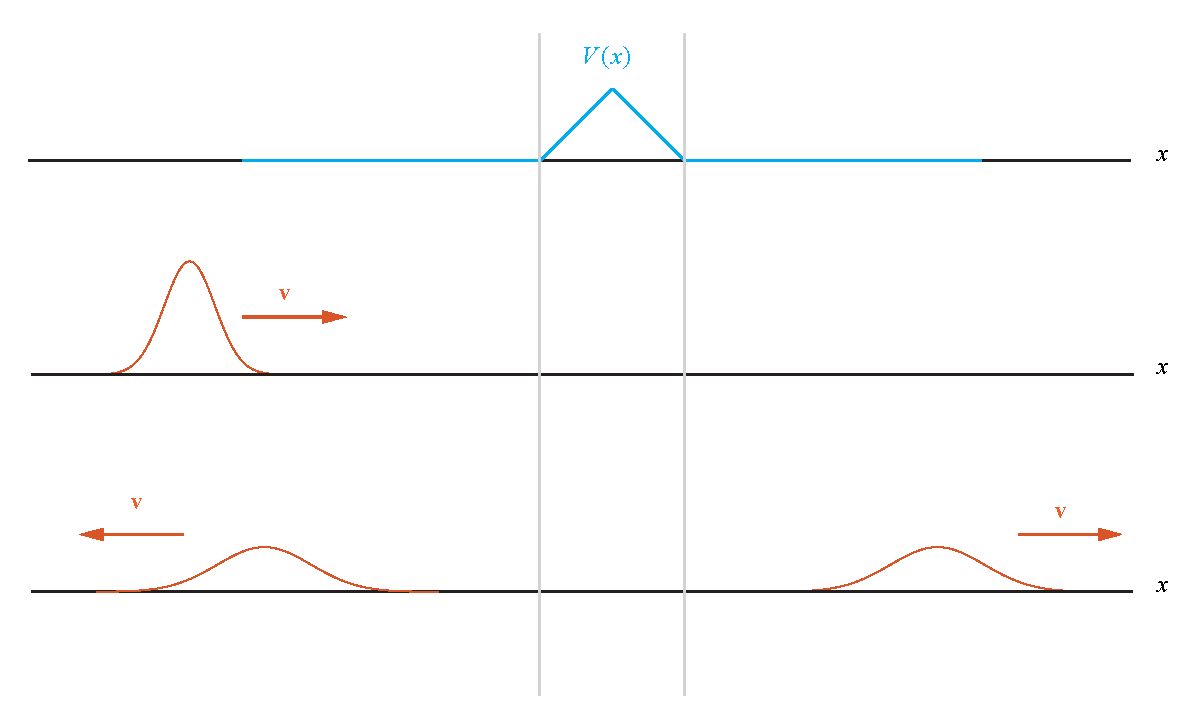
\includegraphics[width=14cm]{./figures/QM03.pdf}
\caption{波包遇到三角形势垒后的散射.} \label{QM0_fig3}
\end{figure}

经典力学中,若粒子匀速入射到如图所示的势能(叫做势垒)上,如果粒子的初始动能小于势垒的最大值,则粒子将会原路返回,若粒子初始动能大于势垒的最大值,则粒子将继续前进.在量子力学中,无论波包以什么初速度入射,波包都会被分为两个不同方向运动的波包,但两个波包的相对大小取决于初始速度.

\subsection{波的叠加}
为什么要用波函数来描述粒子?因为波的一个重要特点就是可以叠加.如果一个波包是薛定谔方程的解,且另一个波包也是薛定谔方程的解,那这两个波包叠加(即把两个波函数相加)后仍然是薛定谔方程的解.例如:两个不同方向运动的波包相遇然后远离.注意这里两个波包并不代表两个粒子,而是代表一个粒子有可能在一个波包的位置被观测到也有可能在另一个被观测到.

\subsection{能量本征态}
在经典力学中,要测量一个粒子的能量,我们只需要先观测其速度,则能量等于质量乘以速度平方除以二再加上该位置的势能.量子力学中,测量波包的能量会得到什么结果呢?这时候我们需要薛定谔方程的另一个用途:对某个势能,我们能解出一些(往往是无穷多个)特殊的波函数,称为本征函数或者本征态.如果粒子的波函数恰好是一个能量本征态,那么测量其能量会得到唯一确定的值(先不讨论用什么方法测)叫能量的本征值.每个本征态对应唯一一个本征值.这些本征态会随时间做简单的周期性变化.

要测量任意波包(波函数)的能量,我们可以想办法用不同的能量本征态叠加来凑出所需波函数,例如第一个本征态乘以常数 C1 加上第二个本征态乘以常数 C2 等,这叫波函数的线性叠加.如果对这个波包测量能量,测到第 i 个能量本征值的概率等于 Ci 的平方.也就是说,某个能量本征态占总波函数的比例越多,越有可能测出对应的能量本征值.

% 未完成:画出以上各例中能量本征态的图像.

\begin{figure}[ht]
\centering
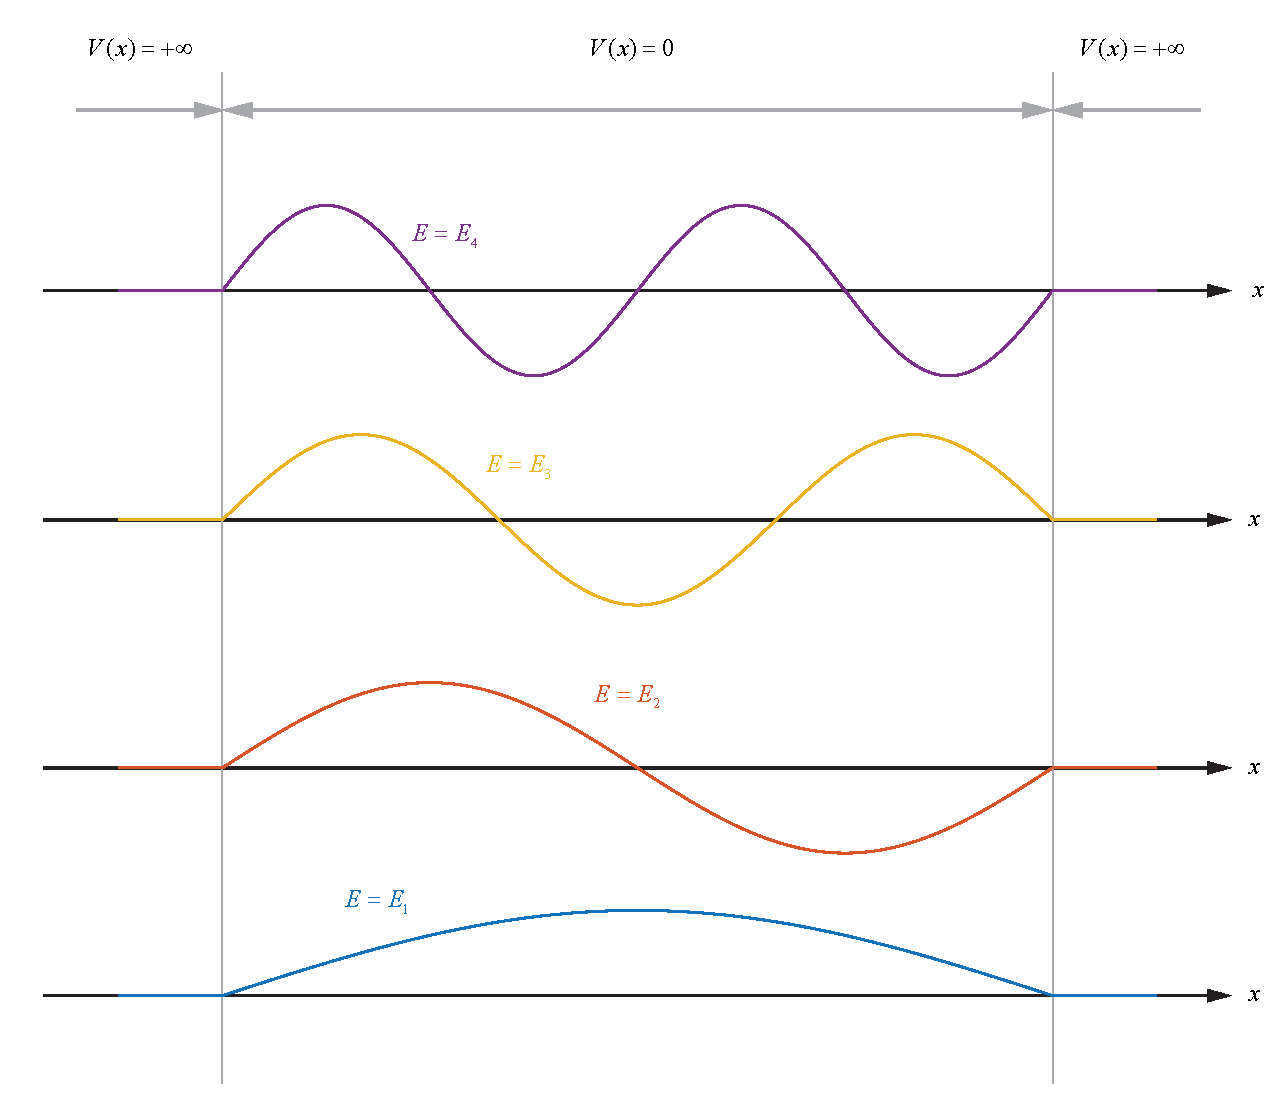
\includegraphics[width=14cm]{./figures/QM04.pdf}
\caption{无限深势阱的一些波函数能量本征态,每个能量 $E_i$ 叫做一个能级,共有无穷多个能级,将这些本征态叠加就能获得任何波函数例如波包.} \label{QM0_fig4}
\end{figure}

\subsection{测量理论}

事实上,不仅是能量,量子力学中的任何物理量的测量都是由以上方法求出.例如动量的本征态是平面波,位置的本征态是一个无穷窄的波包(其描述的粒子只可能出现在某点).如果对一个波包测量某物理量的本征值,就计算出各个本征态占波包的比例 Ci,测量到第 i 个本征值的可能性就是 Ci 的平方.

这里有一个条件是任何物理上可能存在的波包都可以由任何测量量的本征态叠加而成,这叫做本征态的完备性.

测量理论是另一个量子力学的公设.

\subsection{连续本征值与离散本征值}
上面我们提到一个物理量往往有无穷多个本征波函数.一些情况下我们求出的本征波函数对应的值是不连续的(如无限深势阱中的能量本征态),而另一些情况下则是连续的(如动量的本征态总是连续的).经典物理世界中这些物理量都是连续的,而量子中的物理量会出现离散的情况.“量子” 这个词的来源(表示一份一份的).

\subsection{不确定性原理}

\begin{figure}[ht]
\centering
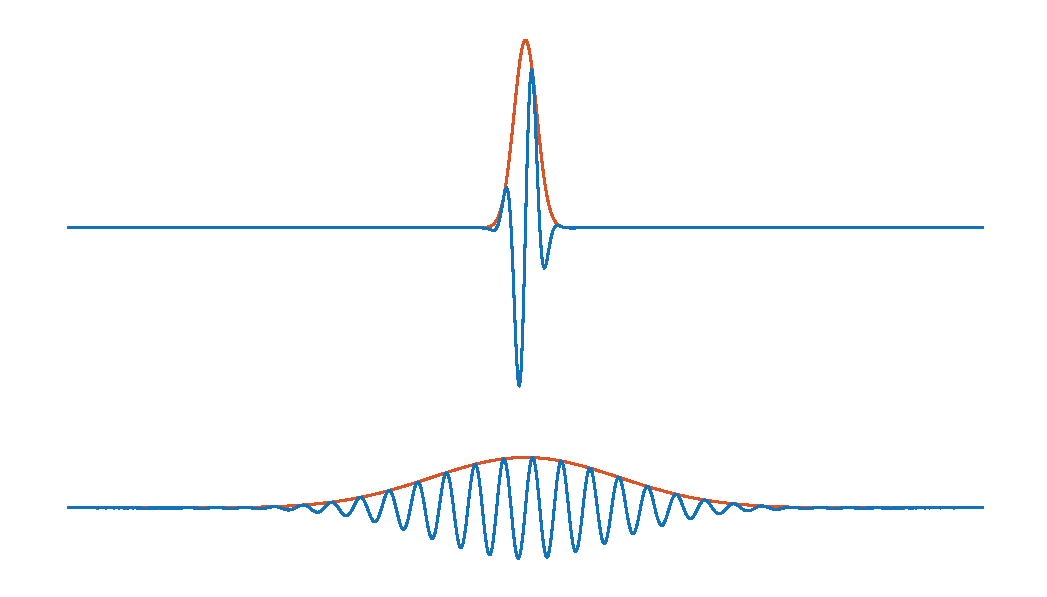
\includegraphics[width=14cm]{./figures/QM05.pdf}
\caption{波包越短,频率就变得越模糊,波包越长,频率就变得更精确.} \label{QM0_fig5}
\end{figure}

不确定行原理是说,我们无法既准确测量粒子的位置和动量(如果你没听说过动量,可以先理解为速度).上文提到位置的本征态是一个无限窄的波包,对应本征值为该波包的位置(坐标).动量的本征态恰恰相反,是一个无限长的波(某个频率的 sin/cos 函数,称为平面波).动量的征值为平面波的频率.

如果波包很窄(但不是无限窄),那么要测量位置,我们只需要使用波包中心附近的一些位置本征态就可以叠加出待测的波包,所以测量结果也只可能离波包中心较近.但在测量动量时,由于这个波包和平面波一点都不像,我们需要非常多的不同频率的平面波叠加才能得到这个波包(为什么无限长的平面波相加能得到有限长的波包?这是数学上一个非常有趣的结果,叫做傅里叶变换.)

另一种情况是,如果波包很长但不是无限长(想象绳子的一段连续上下抖了许多下才停下来),那么将波包看起来与某个频率的平面波十分相似.在测量位置时,我们需要将许多不同坐标的位置本征函数叠加得到波包,那测得的坐标就可能在很大的范围内出现.而测量动量时,我们只需要使用某个频率附近的一些平面波,所以测得的动量(与频率成正比)也都很接近中心频率对应的动量.

